%@AUTHOR: Cardel
%Configuracion del documento

\documentclass{beamer}
\usetheme{Rochester}

\usepackage{graphicx}
\usepackage[utf8]{inputenc}
\usepackage[spanish]{babel}
\usepackage{ragged2e}
\usepackage{colortbl}
\usepackage{color}
\definecolor{naranja}{rgb}{1,0.5,0} % valores de las componentes roja, verde y azul (RGB)
\definecolor{rojo}{rgb}{1,0,0}
\definecolor{SteelBlue}{rgb}{0.3,0.5,0.7}
\usepackage{listings}
\usepackage{listingsutf8}
\usepackage{float}
\usepackage{amsmath, amsthm, amssymb}
\lstset{ %
  basicstyle=\scriptsize,           % the size of the fonts that are used for the code
  numbers=none,
  numberstyle=\footnotesize,          % the size of the fonts that are used for the line-numbers
  numbersep=4pt,                  % how far the line-numbers are from the code
  backgroundcolor=\color{white},      % choose the background color. You must add \usepackage{color}
  breaklines=true,                % sets automatic line breaking
  breakatwhitespace=false,        % sets if automatic breaks should only happen at whitespace
  title=\lstname,                   % show the filename of files included with \lstinputlisting;{}
  extendedchars=false,
  inputencoding=utf8, 
}

%Adicionales


\author{Carlos Andr\'es Delgado S.} 
\title{Arquitectura de computadores I }
\subtitle{Introducción \\ carlos.andres.delgado@correounivalle.edu.co}
\institute{Facultad de Ingeniería. Universidad del Valle}
%Transparencia
\setbeamercovered{transparent}

%LOGO Univalle
\pgfdeclareimage[height=1.4cm]{logo}{imagenes/univalle}
\logo{\pgfuseimage{logo}}

%Para que en cada seccion aparezca la tabla de contenido
\AtBeginSection[]{
	\begin{frame}
	\frametitle{Contenido}
	\tableofcontents[currentsection]
\end{frame}
}

\date{Agosto de 2017}
\newcommand{\grad}{\hspace{-2mm}$\phantom{a}^{\circ}$}
\begin{document}

	\begin{frame}
		\titlepage	 		
	\end{frame}
	\begin{frame}
 		\frametitle{Contenido}
		\tableofcontents
	\end{frame}
	


\section{Introducción a los computadores}

	\begin{frame}
 		\frametitle{Introducción a los computadores}
		\begin{block}{El computador}
		Según el autor del \cite{stallings} un computador es: \\
		\textit{Máquina digital electrónica programable para el tratamiento automático de la información, capaz de recibirla, operar sobre ella mediante procesos determinados y suministrar los resultados de tales operaciones}
		\end{block}
	\end{frame}

	\begin{frame}
 		\frametitle{Introducción a los computadores}
		\begin{block}{Definiciones}
		\begin{itemize}
			\item \textbf{Arquitectura del computador:} Se refiere a todos los atributos visibles por un programador del sistema
			\item \textbf{Organización del computador:} Se refiere a las unidades operacionales y las interconexiones para realizar operaciones de la arquitectura
		\end{itemize}
		\end{block}
	\end{frame}
	\begin{frame}
 		\frametitle{Introducción a los computadores}
		\begin{block}{Motivación}
		¿Por qué estudiar arquitectura de computadores?
		\begin{itemize}
			\item Diseñar mejores programas de base
			\item Optimizar programas
			\item Construir computadoras
			\item Evaluar desempeño
			\item Entender la relación entre poder de cómputo, espacio y costos
		\end{itemize}
		\end{block}
	\end{frame}


	\begin{frame}
 		\frametitle{Introducción a los computadores}
		\begin{block}{Motivación}
\begin{figure}[H]
\centering
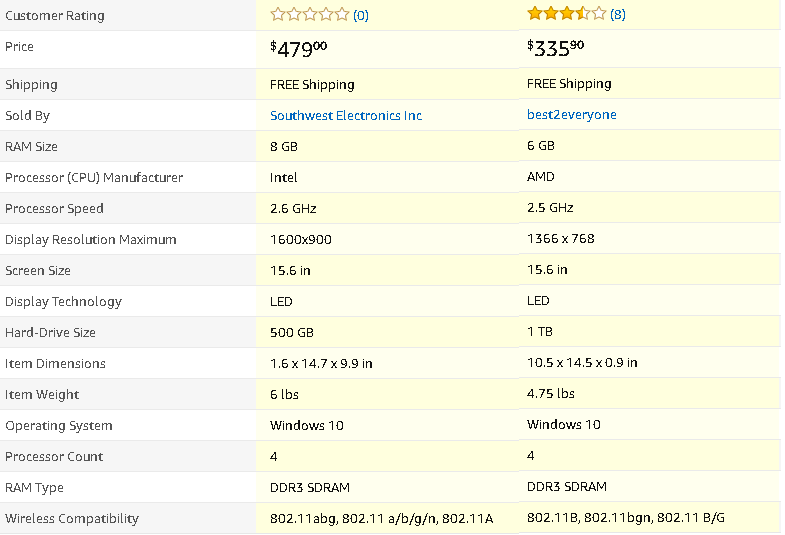
\includegraphics[scale=0.35]{imagenes/pc1.png}
\caption{Computadores en venta. Tomado de amazon.com}
\end{figure}

		\end{block}
	\end{frame}
	
	
	\begin{frame}
 		\frametitle{Introducción a los computadores}
		\begin{block}{Motivación}
\begin{figure}[H]
\centering
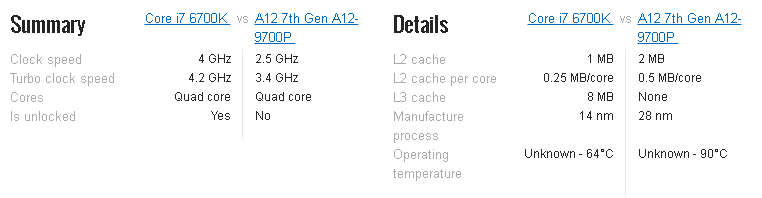
\includegraphics[scale=0.5]{imagenes/pc2.png}
\caption{Los procesadores. Tomado de cpuboss.com}
\end{figure}

		\end{block}
	\end{frame}

	\begin{frame}
 		\frametitle{Introducción a los computadores}
		\begin{block}{Motivación}
		Algunos términos:
		\begin{itemize}
			\item \textbf{Hertz}: Ciclos de reloj por segundo. 
			\item \textbf{Byte}: Unidad de almacenamiento.
			\item \textbf{Word}: Palabra (cantidad de bits que se pueden mover dentro de una CPU)
		\end{itemize}
		\end{block}
	\end{frame}

	\begin{frame}
 		\frametitle{Introducción a los computadores}
		\begin{block}{Motivación}
		Medidas de capacidad y velocidad
		\begin{itemize}
			\item \textbf{Kilo (K)}: $10^3$ y $2^{10}$
			\item \textbf{Mega (M)}: $10^6$ y $2^{20}$
			\item \textbf{Giga (G)}: $10^9$ y $2^{30}$
			\item \textbf{Tera (T)}: $10^{12}$ y $2^{40}$
			\item \textbf{Peta (P)}: $10^{15}$ y $2^{50}$
		\end{itemize}
		Si hablamos de velocidad estamos en unidades de 10 y de capacidad en unidades de 2.
		\end{block}
	\end{frame}	
	
	\begin{frame}
 		\frametitle{Introducción a los computadores}
		\begin{block}{Motivación}
		Medidas de capacidad y velocidad
		\begin{itemize}
			\item \textbf{1KHz}: 1000Hz
			\item \textbf{1MHz}: 1000000Hz o 1000KHz
			\item \textbf{1KB}: $2^{10}$Bytes = 1024 bytes
			\item \textbf{1GB}: $2^{30}$Bytes = 1024 MB
			\item Las palabras (Word) suelen ser unidades de transferencia fija: 8 bits, 16 bits, etc.
		\end{itemize}
		\end{block}
	\end{frame}		
	
	\begin{frame}
 		\frametitle{Introducción a los computadores}
		\begin{block}{Motivación}
		En el caso de la velocidad del procesador $F$ en Hertz, podemos conocer el tiempo de ciclo de reloj $T$ con esta formula:
		\begin{equation*}
		T = \frac{1}{F}
		\end{equation*}
		Ejemplo, un procesador que trabaja a 133MHz, tiene un tiempo de ciclo de reloj de 7.52 nanosegundos
		\end{block}
	\end{frame}	
\section{Estructura y función}


	\begin{frame}
 		\frametitle{Estructura y función}
		\begin{block}{Definiciones}
		\begin{itemize}
			\item \textbf{Estructura:} Como están interrelacionados los componentes
			\item \textbf{Función:} La operación de cada uno de los componentes como parte de una estructura
		\end{itemize}
		\end{block}
	\end{frame}

	\begin{frame}
 		\frametitle{Estructura y función}
		\begin{block}{Vista funcional del computador}
\begin{figure}[H]
\centering
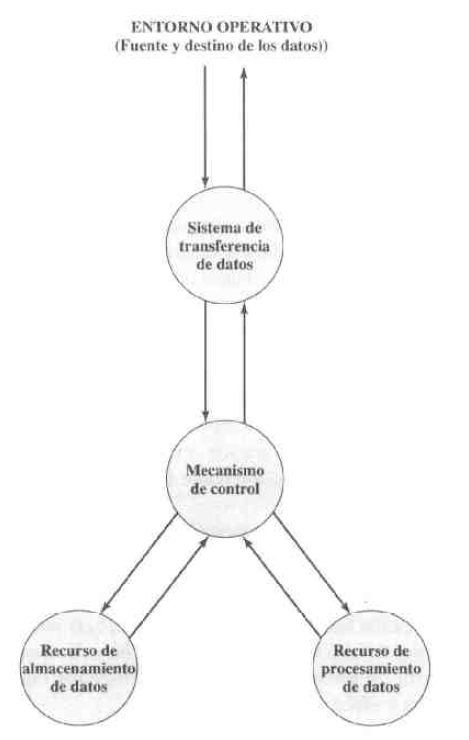
\includegraphics[scale=0.3]{imagenes/pc3.png}
\caption{Vista funcional. Tomado de \cite{stallings}}
\end{figure}
		\end{block}
	\end{frame}

	\begin{frame}
 		\frametitle{Estructura y función}
		\begin{block}{Vista funcional del computador}
		Un computador debe ser capaz de:
		\begin{itemize}
			\item Procesar datos
			\item Almacenar datos
			\item Transferir datos
			\item Debe existir un control de estas 3 operaciones
		\end{itemize}
		\end{block}
	\end{frame}
	
	\begin{frame}
 		\frametitle{Estructura y función}
		\begin{block}{Función del computador}
\begin{figure}[H]
\centering
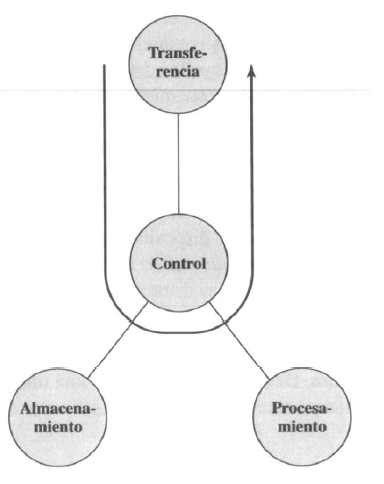
\includegraphics[scale=0.4]{imagenes/pc4.png}
\caption{Transferencia de datos. Tomado de \cite{stallings}}
\end{figure}
		\end{block}
	\end{frame}
	
	\begin{frame}
 		\frametitle{Estructura y función}
		\begin{block}{Función del computador}
\begin{figure}[H]
\centering
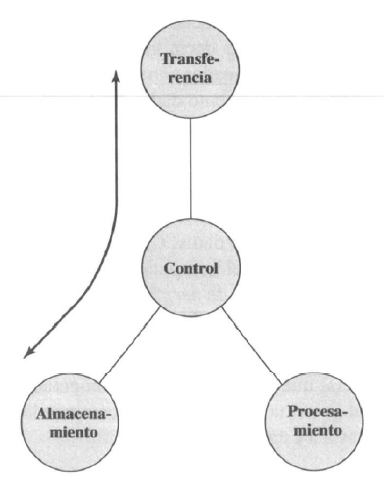
\includegraphics[scale=0.4]{imagenes/pc5.png}
\caption{Almacenanmiento de datos. Tomado de \cite{stallings}}
\end{figure}
		\end{block}
	\end{frame}
	
	\begin{frame}
 		\frametitle{Estructura y función}
		\begin{block}{Función del computador}
\begin{figure}[H]
\centering
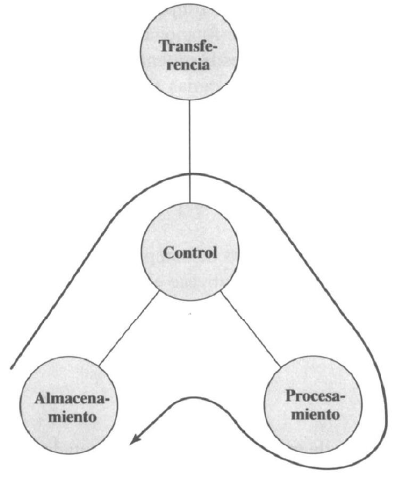
\includegraphics[scale=0.4]{imagenes/pc6.png}
\caption{Procesamiento de datos. Tomado de \cite{stallings}}
\end{figure}
		\end{block}
	\end{frame}
	
		\begin{frame}
 		\frametitle{Estructura y función}
		\begin{block}{Función del computador}
\begin{figure}[H]
\centering
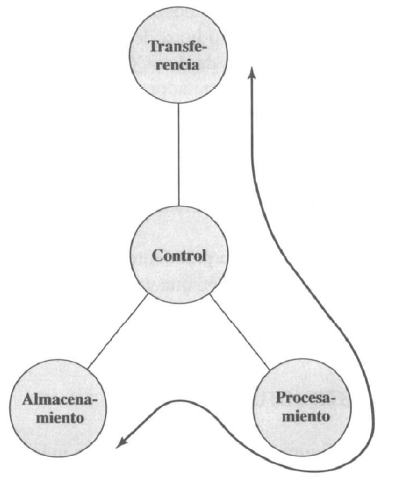
\includegraphics[scale=0.4]{imagenes/pc7.png}
\caption{Transferencia de datos E/S. Tomado de \cite{stallings}}
\end{figure}
		\end{block}
	\end{frame}	
	\begin{frame}
 		\frametitle{Estructura y función}
		\begin{block}{Estructura}
\begin{figure}[H]
\centering
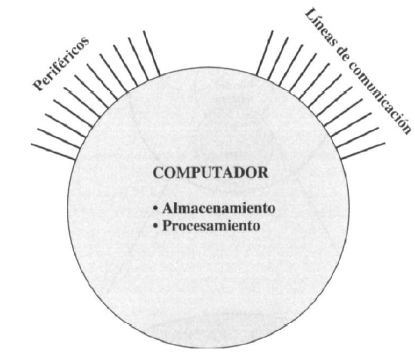
\includegraphics[scale=0.45]{imagenes/pc8.png}
\caption{El computador. Tomado de \cite{stallings}}
\end{figure}
		\end{block}
	\end{frame}
	\begin{frame}
 		\frametitle{Estructura y función}
		\begin{block}{Estructura}
\begin{figure}[H]
\centering
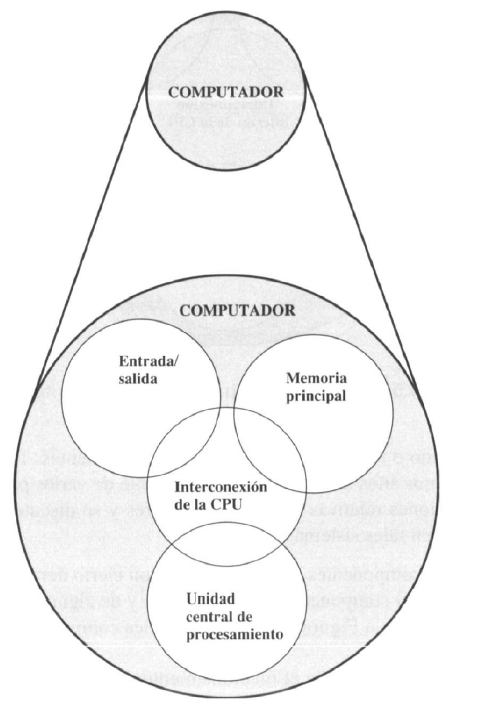
\includegraphics[scale=0.27]{imagenes/pc9.png}
\caption{El computado nivel superior. Tomado de \cite{stallings}}
\end{figure}
		\end{block}
	\end{frame}	
		
	\begin{frame}
 		\frametitle{Estructura y función}
		\begin{block}{Estructura}
		La estructura interna del computador está compuesta por:
		\begin{itemize}
			\item Unidad Centra del Procesamiento (CPU)
			\item Memoria principal
			\item E/S
			\item Sistema de interconexión
		\end{itemize}
		\end{block}
	\end{frame}

	\begin{frame}
 		\frametitle{Estructura y función}
		\begin{block}{El computador}
\begin{figure}[H]
\centering
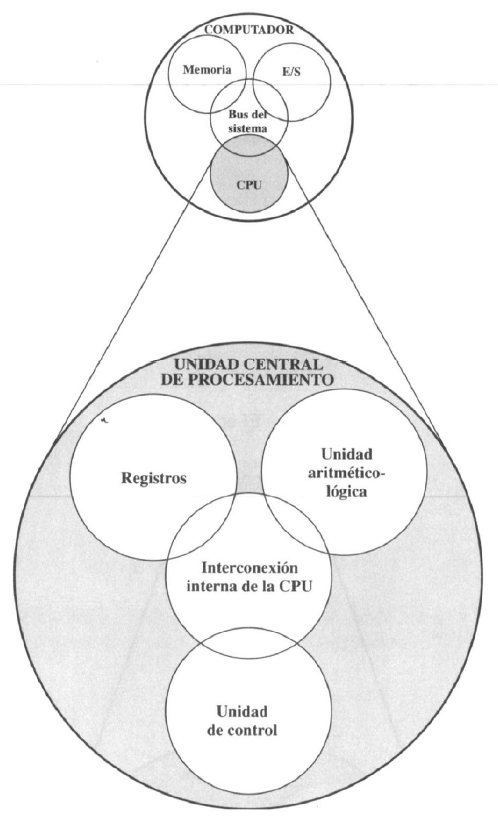
\includegraphics[scale=0.25]{imagenes/pc10.png}
\caption{La CPU. Tomado de \cite{stallings}}
\end{figure}
		\end{block}
	\end{frame}
	\begin{frame}
 		\frametitle{Estructura y función}
		\begin{block}{Estructura}
		La unidad central de procesamiento (CPU) está compuesta por:
		\begin{itemize}
			\item Unidad de control
			\item Unidad aritmético-lógica (ALU)
			\item Registros
			\item Interconexiones
		\end{itemize}
		\end{block}
	\end{frame}
	

	
	\begin{frame}
 		\frametitle{Estructura y función}
		\begin{block}{El computador}
\begin{figure}[H]
\centering
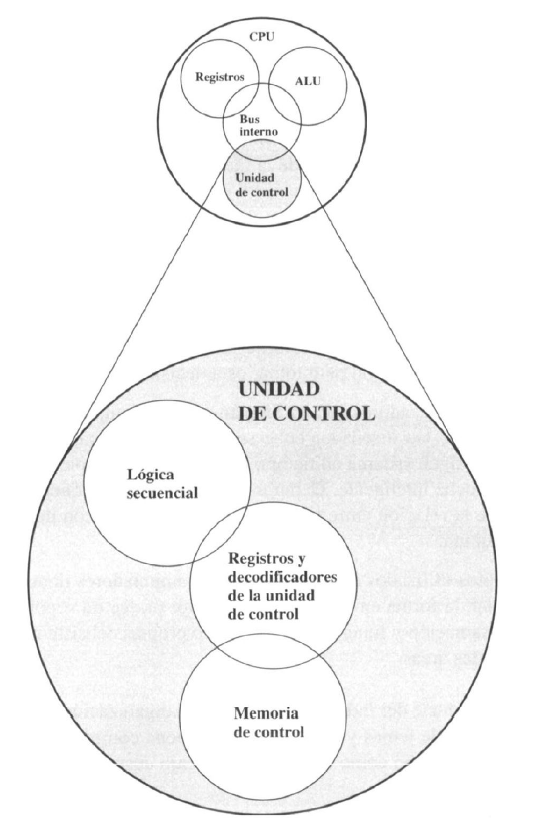
\includegraphics[scale=0.25]{imagenes/pc11.png}
\caption{La unidad de control. Tomado de \cite{stallings}}
\end{figure}
		\end{block}
	\end{frame}	

	
\begin{frame}[allowframebreaks]
  \frametitle{Referencias}
  
    \bibliographystyle{apalike}
    \bibliography{biblio}
\end{frame}


\begin{frame}
	\frametitle{¿Preguntas?}
	\centering
	Próximo tema: \\Evolución y desempeño del computador (Capitulo 2)
\end{frame}					
			

\end{document}